\documentclass[10pt,twocolumn,letterpaper]{article}

\usepackage{cvpr}
\usepackage{times}
\usepackage{graphicx}
\usepackage{algorithm}
\usepackage{algorithmic}
\usepackage{url}
\usepackage{hyperref}



\cvprfinalcopy % *** Uncomment this line for the final submission

\def\cvprPaperID{****} % *** Enter the CVPR Paper ID here
\def\httilde{\mbox{\tt\raisebox{-.5ex}{\symbol{126}}}}

% Pages are numbered in submission mode, and unnumbered in camera-ready
\ifcvprfinal\pagestyle{empty}\fi

\begin{document}
 
\title{Using Bayesian Networks to Predict Change Sets in an IT System}

\author{Sarah Nadi\\snadi@uwaterloo.ca\\University of Waterloo\\ Ontario, Canada}        
\thispagestyle{empty}
\maketitle


\begin{abstract} 
When change one component in an IT system, an analyst must be careful not to negatively impact any of the other system components. Detecting the complete
change set (all those components that need to be changed to avoid any side effects) is therefore very important. Given historic information about how different
components of a system change together, we build a Bayesian network that can be used to predict this change set. Given an initial component to be changed in
the system, the posterior probability of the other components changing can be calculated using the network. In this paper, we experiment with different
techniques for building the Bayesian network based on the data available, and report on their predictive power in terms of recall and precision.
\end{abstract} 



\section{Introduction}
\label{intro}

Change is inevitable in any Information Technology(IT) system. New features are added, different configurations are used, upgrades are introduced and new
software and hardware are added. In a large system, such changes can cause other parts of the system to malfunction without the ability of the analyst to
foresee this side effect. Accordingly, we need to ensure that we consider the impact of changes before they are implemented, and make sure we adjust the
potentially affected components accordingly while implementing the change. This leads to the process of change set detection which is finding all the
components of the system that need to be included in your change set. The change set is the set of components that need to be changed to avoid any side
effects. 

Many of the organizations with large and sophisticated IT systems employ a Configuration Management Database (CMDB) to help them manage these systems.
The CMDB keeps track of all the components in a system, how they are related, as well as all the changes that have occurred to them. Any component in the CMDB
is called a Configuration Item (CI). In previous work~\cite{nadi2010}, we mined the CMDB repository for historical co-changes, and used the mined correlations
to predict change sets. That is, given an initial CI that is going to change, we predict what other CIs might need to be changed as well. We obtained really
promising results in terms of recall and precision (69.8\% and 88.5\% respectively). 

In this paper, we wish to examine the same problem, but from a Bayesian perspective. Instead of looking at pairwise historical co-changes of CI, we would like
to consider all the changed CIs, and learn the relationships between them. That is, given a set of observations about how different CIs change
together, can we deduce the relationships between them that would allow us to predict future change sets. Accordingly, we explore the different ways a Bayesian
network can be constructed from the data we have, and then test the predictions produced by querying this network to examine the obtained recall and precision.
We hope that we can obtain better results using Bayesian networks since they are not limited to pairwise comparisons. 

The rest of this paper is organized as follows. Section~\ref{sec:bg} provides the background information necessary for this work. It explains the nature of
CMDBs, Bayesian networks, and the tools we used for analyzing Bayesian networks. Section~\ref{sec:constructing} then presents the techniques we used to build
our Bayesian network. This includes how we process the data, and build the different Bayesian networks accordingly. Section~\ref{sec:setup} details the
setup we use for our experiments, and Section~\ref{sec:results} provides the results obtained. Section~\ref{sec:discussion} provides a general insight to the
results, and future work that could be done to improve them. Section~\ref{sec:concl} concludes this paper.


\section{Background}
\label{sec:bg}

\subsection{CMDBs and Change Sets}
The repository of information we are using is the Configuration Management Database (CMDB)~\cite{itil}. The CMDB is useful in Enterprise IT Management (EITM)
since it provides information about the various critical components in a system including hardware, software, and services provided by the company. It records
the configuration of these items, their change history, their incident history, as well as the relationships between them. Each item stored in the CMDB is
referred to as a Configuration Item (CI). Figure~\ref{fig:cmdbExample} shows an example CMDB to illustrate the concepts of CIs and relationships.

A CMDB provides a basis for decision making processes such as Incident Management, Change Management, etc.  In this paper, we focus on the process of Change
Management, and in particular, on the problem of change set detection. A \textit{change} is the addition, modification, or removal of anything that could affect
on IT services. A poorly planned change may lead to a fault in the system. Accordingly, when one wants to change a CI is the system, other CIs that might
need to be changed as well must be correctly identified. We refer to the set of CIs that will need to be modified for the change to be complete ias the
\textit{change set}.

\begin{figure}[!t]
\centering
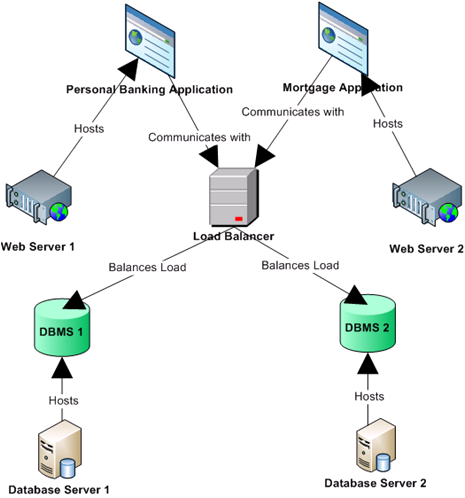
\includegraphics[width=7cm]{cmdbExample.PNG}
\caption{An IT System Stored in a CMDB. Each item shown is a CI, and CIs are tied through different relationship types}
\label{fig:cmdbExample}
\end{figure}

\subsection{Bayesian Networks}

Bayesian Networks, first introduced by Pearl~\cite{pearl1988probabilistic} are a type of probabilistic graphical models. Each node in the network
represents a random
variable, and nodes are connected through edges which represent probabilistic dependencies~\cite{benbayesian}. A Bayesian network is a Directed
Acyclic Graph (DAG), and is essentially defined by two aspects: the structure of the graph and the Conditional Probability Tables (CPTs) probabilistically
relating connected nodes. In our work, a node in the Bayesian network would be a CI which can take values {``true'',``false''} to donate the probability of it
changing or not. The CPTs would essentially give the probability of one CI changing given its parents' values.

Given a set of data consisting of observations for our variable space, machine learning techniques can be used to estimate the network. If the structure of the
network is known, and we have full observability (i.e we can observe values for each variable), then learning the CPTs can be achieved through
Maximum-likelihood estimation (MLE)~\cite{benbayesian}. MLE tries to maximize the log likelihood of the the training data which can simply be done by
calculating the frequency of occurrence of the values of each variable given its parents. If the structure is known, but we only have partial observability
(i.e., missing data), then we can use a variation of MLE which is the Expectation Maximization algorithm~\cite{dempster1977maximum}. If the structure is not
known in
the first place, then searching through the model space, and calculating network scores for each produced network is necessary. The simplest algorithm for this
is a Greedy search algorithm~\cite{friedman1996learning}.

While searching for the best network that fits the training data, scores are needed for the produced networks in order to know which one is the best one. There
are several types of scores that have been proposed in the literature. Two of the commonly used scores are the Minimum Description Length (MDL)
score~\cite{rissanen1986stochastic} and the BDe score~\cite{heckerman1995learning}. The MDL score is based on finding the length of data required to store a
network. It tries to balance the complexity of the induced network with the degree of accuracy of which the network represents the frequencies in the training
data. Therefore, the lower the MDL score of a network, the better it is. The BDe score is proportional to the posterior probability of each network structure
being scored, given the data. Accordingly, we are searching for the network that maximizes this probability. For large data sets, both metrics score
structures similarly~\cite{friedman1996learning}. 

\subsection{Bayesian Network Tools}

There are many machine learning and Bayesian analysis tools available. In this work, we use three of these tools which we briefly describe
below.

\subsubsection{WEKA}

WEKA~\cite{hall2009weka} is a Java toolbox for machine learning. It provides different algorithms for classification and clustering as well as other machine
learning problems. It has Bayesian learning techniques for classification problems. Additionally, it provides explorations tools for Bayesian
Networks, and allows the user to learn the structure and CPTs of a Bayesian Network. IN terms of learning CPTs, one of the algorithms WEKA implements is
the SimpleEstimator algorithm~\cite{witten2005data} implemented which we use in our work. This simply estimates the probability values on edges based on
the frequency values of each variable given its parents in the training set.

\subsubsection{Banjo}
Banjo~\cite{banjotool} is a tool written in Java which infers the structure of a Bayesian network given training data. It has two different search algorithms:
Greedy and Simulated Annealing. Banjo uses the BDe metric to compute a network's score, and produces the highest scoring network found. We used the Greedy
search algorithm in our experiments.

PIC STILL NEEDS WORK

\begin{figure*}[!t]
\centering
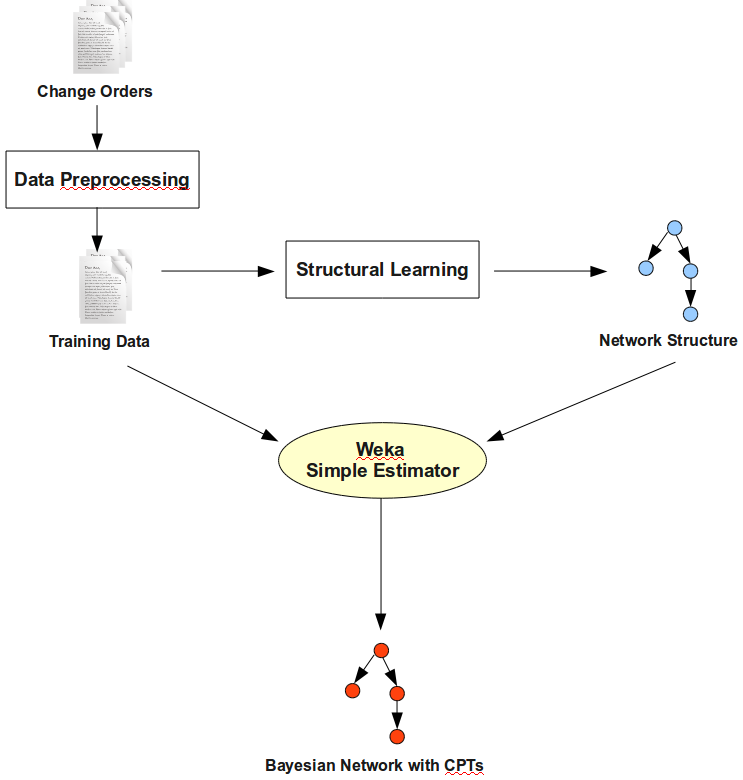
\includegraphics[width=15cm]{graphics/constructingmodel.png}
\caption{Building the Bayesian Network}
\label{fig:process}
\end{figure*}

\subsubsection{JavaBayes}

JavaBayes is a Java tool for calculating marginal probabilities and expectations in a Bayesian network. In a network, nodes can be set to be observed, and then
the posterior probability of the remaining nodes can be calculated using Bayes theorem. This is the functionality we need here since the CI that will be
changed will be considered as observed to be ``true'', and then we need to calculate the posterior of the remaining CIs given this observation.


\section{Constructing the Bayesian Network}
\label{sec:constructing}

Before constructing the Bayesian Network, we first have to process and prepare the data we have. In order to construct a Bayesian network to use for
predictions there are two steps involved. First, determining the structure of the actual network, and then estimating the Conditional Probability Tables
(CPT). Section~\ref{sec:data} first explains the data set available to us, and the data preprocessing involved before building the network.
Section~\ref{sec:structure} then explains the different techniques we experimented with to build the network structure. Section~\ref{sec:cpt} shows the last
step to build the network which is estimating the CPTs. Figure~\ref{fig:process} shows this overall process.

\subsection{Data Preprocessing}
\label{sec:data}

\subsubsection*{Data Size}
The data set available to us in the sample CMDB we have is from three years, and has 7,999 distinct CIs, and 27,305 change orders. This amount of data
was infeasible to work with as no tool could handle such a large amount of variables in a Bayesian network. For the purposes of this project, which is mainly to
experiment with Bayesian techniques for change set prediction, it is sufficient to choose a small representative subset of the data. Accordingly, in order to be
able to test things properly, we used observations from three months data from January 1, 2008 to March 31, 2008 to build the model. However, even in such a
short period, there were already 2,841 distinct CIs appearing and 2,229 observations (i.e. change orders). Therefore, we needed to perform further data
preprocessing. 

First, we removed all CIs that have changed less than 12 times within this time frame  (i.e were associated with less than 12 different change orders in our
training observations). There is no particular reason for choosing 12 as a cut off. It simply gave a feasible data set to deal with. This yielded 120 distinct
CIs. Then, in order to slightly increase our variable space to include other related CIs, we found all the parent CIs related to these 120 CIs from the CMDB
perspective. Adding the related parent CIs, we now had a set of 241 CIs. However, some of the added parent CIs may not be in the original set of 2,841 CIs.
Accordingly, we just kept CIs that appeared more than 12 times or were in the set of related CIs. This provided us our final data set of 170 CIs which we use
throughout our models for fair comparison. Additionally, filtering out CIs meant filtering out some of the change orders that did not have any CIs satisfying
our criteria (i.e. all the CIs that changed in them were outside our 170 CI set). This led to us having 1,305 change orders instead of 2,229 which was more
manageable set. Accordingly, our training data set consisted of 170 variables (CIs), and 1,305 observations (change sets).  TRAINING?

\subsubsection*{Data Format}
\label{sec:format}

In the CMDB, a Change Order has several fields including the requester, the assignee, the start date of the change, the description and the change set field
(called the `Configuration items' fields). Of the fields in a change order, we use only the change set field. The advantage of only using this one field is that
change sets are easy to extract and easy to understand. In terms of an observation, CIs were either marked as ``true'' or ``false'' indicating whether they
have changed or not. Each observation initially consisted of all the CIs in our data set marked as ``false''. For each change order in the training set, we
would
mark each CI appearing in the ``Configuration Items'' field as true, while all those not appearing were left as ``false''. Therefore, the set of training
data consisted of an observation entry for each change order with the CIs marked as ``true'' or ``false'' accordingly.

\subsection{Network Structure}
\label{sec:structure}
There were essentially three different ways in which we could estimate the structure of the network. We, thus, built a Bayesian Network using each technique to
be able to compare their performance.


\subsubsection{Method 1 (Banjo)}
\label{sec:model1}

For the first method, we used Banjo to learn the structure of the Bayesian network from the training data. We use the Greedy searching algorithm implemented
there. Banjo produced five different top-scoring networks (having the same score), and we simply chose one of them as the network to be used.

\subsubsection{Method 2 (WEKA Classification)}

Although our research problem as currently defined is not really a classification problem, we want to examine how the network built by the BayesNet classifier
in WEKA will perform. Accordingly, we estimated the structure of the network using the K2 structure learning algorithm implemented in WEKA which is also a
greedy
search based learning algorithm. The default maximum number of parents allowed for any node is one (a Naive Bayesian Network). However, we used a maximum of
five to allow the nodes to be related since there is really no class label in our data set. We could not experiment with other techniques in WEKA because they
do not allow multiple parents.

\subsubsection{Method 3 (CMDB Relationships)}

For the third method, we used the relations existing in the CMDB to infer the structure of the network. We used two
variations for this. The first was to follow the direction of the relationship edges in the CMDB. That is, if there is a relationship edge in the CMDB from A to
B, we will place an
edge in the Bayesian network from A to B. The second was to reverse the direction of the relationship edges in the CMDB. That is,
if there is a relationship edge from A to B in the CMDB, we will place an edge in the Bayesian network from B to A. There was one problem, however, with
the generated networks. Two of the CIs had more than 15 parents to them which means that their CPTs will be intractable to compute. For those two CIs, we simply
removed all their parents to make the computation tractable.

\subsection{Estimating the CPTs}
\label{sec:cpt}

After the structure was determined, we used the SimpleEstimator algorithm~\cite{witten2005data} built in WEKA to calculate the CPTs for all networks. After
setting the data set to be the observations in our training set (an ARFF file), WEKA learned the CPTs for each of the
networks above. This complete network was then saved as an BIF XML file to be used by JavaBayes for general inference as will be explained in the next section.

Additionally, we experimented with the missing data feature in WEKA. WEKA allows the user to specify missing values
for any variable by simply putting a '?' instead of its value. Therefore, instead of putting the CIs that did not appear in a change order as false, we put a
'?' in their place. This seemed closer to practice, because in reality, we are not sure whether this CI actually changed or not. When using Banjo or the CMDB
relationships to estimate the structure of the network, the missing values were only inserted when learning the CPTs. When using WEKA, the missing values were
inserted both to learn the network, and to estimate the CPTs.


\section{Experiment Setup}
\label{sec:setup}

This section explains how we tested the predictions of each of the networks in a way that simulates how an analyst would use the tool in reality. We first
explain how we simulate this behavior, and then explain how we evaluate the predicted CIs. Algorithm~\ref{alg:simulation} summarizes these steps taken to
predict a change order.

\begin{algorithm}[tb]
   \caption{Generating Predictions using the Bayesian Network}
   \label{alg:simulation}
\begin{algorithmic}
   \STATE {\bfseries Input:} $change order$
    \STATE {\bfseries Input:} $Bayesian network$
    \STATE {\bfseries Input:} $threshold$
    \STATE Set $initial CI$ = first CI in changeOrder
    \STATE Set $occurred set$ = $change order$ - $initial CI$
    \STATE Initialize $observed set$ = {$initial CI$}
    \STATE Initialize $predicted set$ = {}
   \REPEAT  
    \STATE Initialize $new predictions$ = {}
    \FOR{$node$ in $BayesianNetwork$}
    \STATE $posterior$ = query $node$ in $Bayesian network$ using Banjo given observed set
    \IF{$posterior > threshold$ and $node$ not in $predicted set$} 
      \STATE Add $node$ to $new predictions$   
    \ENDIF
    \ENDFOR

  \FOR{$prediction$ in $new predictions$}
    \IF{$prediction$ in  $occurred set$}
      \STATE Add $prediction$ to $observedSet$
    \ENDIF
    \ENDFOR
\STATE Add $new predictions$ to $predicted set$

   \UNTIL{$new predictions$ is empty}
\STATE $recall = (predicted set \cap occurred set)/occurred set$
\STATE $precision = (predicted set \cap occurred set)/predicted set$
\end{algorithmic}
\end{algorithm}

\subsection{Change Set Detection Process Simulation}

The change set detection process provided is an iterative, collaborative process between the tool and the analyst. When the tool suggests CIs, the analyst can
accept or reject these CIs (i.e add them to the change set or not). Based on the CIs added to the change set, the analyst can ask the tool for more
suggestions. This is along the lines of ``Now, that I am also going to change these CIs, what else do I need to change?''. This process is explained in more
details by Nadi et al.~\cite{nadi2010}.

To simulate this process for our experiments, we do the following. At this point, we have the Bayesian network ready, and we would like to perform Inference.
More formally, given that a CI will change (our observation), we want to update our beliefs that the other CIs in the network might change as well.
Unfortunately, neither of the two tools previously used provide a general inference engine. We, therefore, use JavaBayes in this step since it accepts
the same XML BIFF format produced by WEKA. [We use a one month testing set where we try to predict all the change orders in April 2008. There was a total of
883 change orders in that month which we use in our testing set. ] - REMOVE?

For each change order, we would take the first CI recorded as the initial CI to change, then we would set that as an observed node, and update
the beliefs of all the nodes (CIs) in the network using JavaBayes. We are basically checking the posterior probability of each CI being ``true'' given our
observation. We used different
cutoff thresholds for the posterior probabilities we would consider. We would then loop on all the updated CIs, and add those that match our threshold criteria
to
the predicted change set. For example a threshold of 0.2 means that only nodes that have a posterior probability greater than 0.2 of having the value ``true''
will be returned. To simulate a real life scenario, we then checked which of these predicted CIs actually lies in the target change set we are trying to
predict. This is similar to an analyst accepting CIs into their change set. These common CIs would then also be marked as observed so that we can predict
what else will need to change given that these CIs are also changing. Again, we would calculate the posterior probability given the new observations, and
continue doing
so until there are no more common CIs. All the CIs that match the threshold criteria (whether accepted by the analyst or not) are part of the predicted
set. These steps (shown in Algorithm~\ref{alg:simulation} would be repeated for each change order.

\subsection{Evaluation Techniques}

We need a way to evaluate the predicted CIs. The recall and precision measures from Information Retrieval are appropriate for this type of evaluation.
Recall measures the proportion of correct CIs retrieved by the system, while precision measures the proportion of suggested CIs that are correct~\cite{van79}.

Similar to Hassan et. al~\cite{hassan2004predicting}, we define the \textit{Predicted Set} (P) as the set of all predicted. We define the \textit{Occurred
Set} (O) as the CIs remaining in the change set after excluding the Initial CI
provided by the analyst (i.e Change Set - Initial CI). The intersection of the predicted set and the occurred set, called $PO$, is the common CIs in both sets.
For each constructed change set, we then calculate the recall and precision values for the predictions according to the following
definitions~\cite{hassan2004predicting}:

\begin{equation}
\label{eqn:recall}
Recall = \frac{|PO|}{|O|}
\end{equation}

\begin{equation}
\label{eqn:precision}
Precision = \frac{|PO|}{|P|}
\end{equation}

If no CIs are predicted (i.e., $P$ and thus $PO$ are empty), precision is defined as 1 since there cannot exist any incorrect predictions in an empty set. On
the other hand, if the size of the change set is 1, and thus the size of the occurred set is 0, recall is defined as 1 since there are no CIs to
predict~\cite{hassan2004predicting}.  

In order to have a single measure that indicates the effectiveness of our predictions, we use the F-measure which is based on van Rijsbergen's effectiveness
measure which combines recall and precision~\cite{van79}. The F-measure is calculated according to Equation~\ref{eqn:f-measure} which gives equal weighting to
recall and precision. The ideal F-measure is 1 where both recall and precision are 1.

\begin{equation}
F = 2 * \frac{precision * recall}{precision +recall}
\label{eqn:f-measure}
\end{equation}

\begin{table*}[h!t!]
\centering
\resizebox{\textwidth }{!}{
\begin{tabular}{ c | c |c ||c | c || c |c ||c | c || c |c ||c| c||c|c||c|c}
\textbf{Threshold} 
& \multicolumn{2}{|c||}{\textbf{Banjo}} 
& \multicolumn{2}{|c||}{\textbf{Banjo Missing}}
&\multicolumn{2}{|c||}{\textbf{WEKA}}
&\multicolumn{2}{|c||}{\textbf{WEKA Missing}}
&\multicolumn{2}{|c||}{\textbf{CMDB}}
&\multicolumn{2}{|c||}{\textbf{CMDB Missing}}
&\multicolumn{2}{|c||}{\textbf{Reversed CMDB}} 
&\multicolumn{2}{|c}{\textbf{Reversed CMDB Missing}}\\
\hline
 & \textbf{Recall} 
& \textbf{Precision}
& \textbf{Recall} 
& \textbf{Precision}
& \textbf{Recall}
& \textbf{Precision}
& \textbf{Recall} 
& \textbf{Precision}
& \textbf{Recall} 
& \textbf{Precision}
& \textbf{Recall} 
& \textbf{Precision}
& \textbf{Recall} 
& \textbf{Precision}
& \textbf{Recall} 
& \textbf{Precision}\\
\hline\hline
0&0.715&0.473&0.715&0.473&0.715&0.473&0.715&0.473&0.715&0.473&0.715&0.473&0.715&0.473&0.715&0.473\\
\hline
0.1&0.649&0.493&0.715&0.473&0.707&0.501&0.715&0.473&0.569&0.470&0.715&0.473&0.583&0.471&0.715&0.473\\
\hline
0.2&0.643&0.501&0.715&0.473&0.704&0.509&0.715&0.473&0.568&0.470&0.715&0.473&0.580&0.470&0.715&0.473\\
\hline
0.3&0.634&0.510&0.715&0.473&0.700&0.519&0.715&0.473&0.568&0.469&0.715&0.473&0.569&0.469&0.715&0.473\\
\hline
0.4&0.624&0.511&0.715&0.473&0.696&0.524&0.715&0.473&0.568&0.469&0.715&0.473&0.568&0.469&0.715&0.473\\
\hline
0.5&0.610&0.500&0.715&0.473&0.682&0.528&0.715&0.473&0.568&0.469&0.715&0.473&0.568&0.469&0.715&0.473\\
\hline
0.6&0.607&0.500&0.715&0.473&0.674&0.529&0.715&0.473&0.567&0.469&0.715&0.473&0.568&0.469&0.715&0.473\\
\hline
0.7&0.595&0.499&0.715&0.473&0.646&0.526&0.715&0.473&0.567&0.469&0.715&0.473&0.568&0.469&0.715&0.473\\
\hline
0.8&0.595&0.499&0.715&0.473&0.627&0.526&0.715&0.473&0.567&0.469&0.715&0.473&0.567&0.469&0.714&0.473\\
\hline
0.9&0.574&0.475&0.715&0.473&0.588&0.489&0.567&0.469&0.567&0.469&0.715&0.473&0.567&0.469&0.712&0.473\\
\hline
1&0.567&1.000&0.567&1.000&0.567&1.000&0.567&1.000&0.567&1.000&0.567&1.000&0.567&1.000&0.567&1.000\\
\end{tabular}
}
\centering
\caption{Summary of Results}
\label{tab:results}
\end{table*}




\section{Results}
\label{sec:results}

\begin{figure}[!t]
\centering
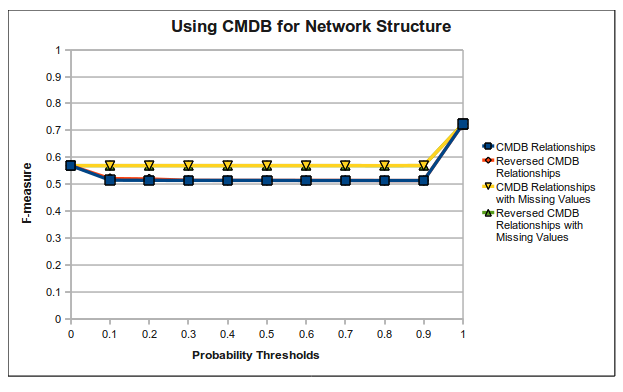
\includegraphics[width=8cm]{graphics/cmdbresults.png}
\caption{F-measure of the different Bayesian networks produced using the CMDB relationships}
\label{fig:cmdbresults}
\end{figure}

For all the networks generated from the different methods explained in Section~\ref{sec:structure}, and following the procedure described in
Section~\ref{sec:setup}, we calculated the average recall and precision for all the change orders in the test set. Based on the average recall and precision
values, we calculated the F-measure. Table~\ref{tab:results} summarizes the recall and precision obtained for all models. For better visualization, we plot the
results from all the networks based on CMDB structure together, and the results from those based on Banjo and WEKA together.

Figure~\ref{fig:cmdbresults} shows the F-measure obtained from the four different networks built based on CMDB relationships for structural information. The
first observation is that reversing the relationship edges did not produce any difference in the results. The curves for the CMDB relationships and the reversed
CMDB relationships are completely overlapping. The same things applies to the curves of CMDB relationships with missing data, and reversed CMDB relationships
with missing data. The second observation here is that denoting CIs that did not appear in the change order as missing data rather than giving them the value
``false'' produced slightly better results. However, the main conclusion from these results is that given each change order, all of the predicted CIs in the
network already had a posterior probability of greater than 0.9. That is why the F-measure is the same for all thresholds (excluding 0), and only
changes when the threshold becomes 0.9. This seems rather strange, and despite the relatively high F-measure, it does not seem that the structure
of these networks is reflective of their relationships in terms of change.

\begin{figure}[!t]
\centering
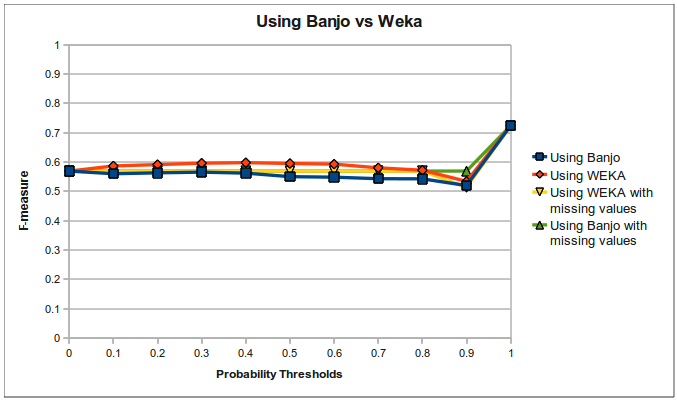
\includegraphics[width=8cm]{graphics/banjowekares.png}
\caption{F-measure from network structures estimated by WEKA versus Banjo}
\label{fig:wekabnj}
\end{figure}

Figure~\ref{fig:wekabnj} compares the F-measure obtained from the graphs whose structure was built using Banjo versus those built using WEKA. It also shows the
effects including missing data in both cases. Surprisingly, it seems that the network built using WEKA has better performance (although only slightly better).
However, marking CIs that have not been changed as unobserved (missing) instead of ``false'' slightly deteriorated the predictive performance. Overall, the
performance of the two networks are very similar which comes as a surprise since WEKA is really a classification engine and assumes that the last variable in
the data is the target class which is not the case in our data. 

We also note when the threshold is 1.0 (i.e no predictions are being made), the recall is not 0 although the precision is 1. This is because there are many
change sets of size 1 which makes the occurred set of size 0, and thus recall being automatically 1. Please refer to Nadi et. al~\cite{nadi2010} for more
details. Additionally, all networks start at the same recall and precision values when the threshold is 0 since simply all 170 CIs are predicted. This is
because in the Bayesian network, the probability of any CI is never really zero. It may be very close to zero, but will never be completely unlikely.



\section{Related Work}
\label{rel-work}

Mirarab et al.~\cite{mirarab2007} investigate the same problem as our work. They build three
different Bayesian Networks, one that is based on package and class dependency information (static relationships), one which is dependent on historical
co-changes, and one which uses both. For the first graph, the initial structure is essentially ``given'' according to the static dependencies, and then the CPTs
are learnt using the importance sampling algorithm proposed by Changhe and Marek~\cite{yuan2003importance}. The way static dependencies are defined in their
case is specific to Java. The third one is essentially the first graph, but updated using the historic change information according to the Expectation
Maximization (EM) algorithm~\cite{dempster1977maximum}. The second was solely based on historic information where the network is build using a greedy structure
 learning algorithm~\cite{friedman1996learning}. The main difference between their work and ours is that their work is on the level of source
code while ours is on a system level.

Zhou et al.~\cite{zhou2008} try to answer a slightly different problem. They do not only look at the probability of other elements changing given a specific
element, they also add features such as authors, change significance levels etc. and try to predict if two elements are co-changes or not accordingly. Thus,
their problem is more of a classification problem where given two elements, and some observed features they try to determine the class as a co-change or not.
They use the K2 algorithm proposed by Cooper et. al~\cite{cooper1992bayesian} to estimate the structure of the Bayesian network, and use the SimpleEstimator
algorithm built in WEKA~\cite{witten2005data}.

\section{Future Work}
\label{sec:future}

There is still some work that needs to be done in this area. First, it would be intersting to experiment with undirected graphs. For our problem, when two CIs,
A and B, occur in the same change order, it is hard to determine whether A caused B to change or B caused A to change. Therefore, using an undirected model,
such as a Markov network could be interesting in this setting. Unfortunately, due to time constraints, we could not experiment with that. Another possible
expansion is to use the CMDB relationships more carefully when determining the structure of the network. Currently, we either add edges to the Bayesian network
following the direction of those in the CMDB or in the reverse direction. It would be interesting to determine which set of relationships semantically make
sense to have the causality relationship in their same direction, and which make sense to have it in the opposite direction. That way, the structure of the
network produced could perhaps be more accurate.

\section{Conclusion}
\label{concl}

In this work, we experimented with Bayesian networks in the context of change set predictions for IT systems. Given the CIs the analyst wants to change in the
system, we can predict what other CIs might need to be changed as well. We built different Bayesian networks based on different information such as CMDB
relationships or using structural learning algorithms such as the Greedy algorithm.


\bibliography{references}
\bibliographystyle{ieee}

\end{document} 


